\section*{1.1}

\subsection*{الف}
با انتخاب یک رشته از مجموعه

\[L = \{a^m b^n c^p d^q \, | \, m + n = p + q\}\]
ما می‌خواهیم یک گرامر بسازیم که بتواند این رشته را تولید کند. بنابراین می‌توانیم گرامر زیر را بسازیم:
\begin{align*}
	S &\to a S d \, | \, A \, | \, B \\
	A &\to C \, | \, a A c \\
	B &\to C \, | \, b B d \\
	C &\to b C c \, | \, \epsilon
\end{align*}
اگر به گرامر نگاه کنیم، می‌بینیم که در هر قاعده، تعداد حروف $a$ و $b$ همیشه با تعداد حروف $c$ و $d$ مطابقت دارد. بنابراین، با انتخاب انتخابات مناسب از قواعد، می‌توانیم هر رشته از $L$ را تولید کنیم.

\subsection*{ب}
برای این بخش، مجموعه رشته‌های ما به شکل زیر است:

\[
L = \{u a w b \, | \, u, w \in \{a,b\}^{*} and |u| = |w|\}
\]
برای این که این رشته‌ها را تولید کنیم، نیاز به گرامری داریم که بتواند حروف $a$ و $b$ را در مواقعی تولید کند که تعداد حروف قبل و بعد از آنها مساوی باشد. بنابراین، می‌توانیم گرامر زیر را بسازیم:
\begin{align*}
	S &\to Ab \\
	A &\to a \, | \, B A B\\
	B &\to a \, | \, b
\end{align*}
این گرامر با توجه به تعداد مساوی حروف در رشته‌های $u$ و $w$، همیشه یک $a$ را در میانه رشته و یک $b$ را در انتهای رشته قرار می‌دهد.

\section*{2.1}

\subsection*{الف}
گرامر زیر را برای توصیف داریم:

\[
(0^{*}10)(\#(0^{*}10))^{*}
\]
در این گرامر، $A$ می‌تواند یا یک $10$ تولید کند یا با تولید $0A$ به حالت توصیف شده برسیم. علاوه بر این، $#$ عملگری است که رشته‌ها را در میانه جدا می‌کند.

\subsection*{ب}
برای این قسمت داریم:

\[
L = \{(a|b)u w \, | \, u, w \in \{a,b\}^{*} \,and\, |u| = |w|\}
\]
از آنجا که رشته یا با $a$ یا با $b$ شروع می‌شود و سپس دوتا دوتا ترکیب‌های یکسان از آنها تولید می‌شود، به توصیف مجموعه فوق می‌رسیم.

\section*{3.1}

\subsection*{الف}

\begin{center}
	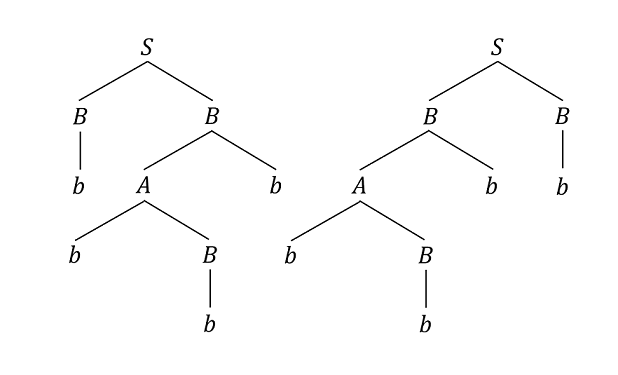
\includegraphics{image1}
\end{center}

برای نشان‌ دادن اینکه گرامر ابهام دارد، می‌توانیم دو درخت مختلف برای یک رشته از گرامر بسازیم. این نشان می‌دهد که گرامر ابهام دارد زیرا برای یک رشته وجود چندین درخت اشتقاق ممکن است.

\subsection*{ب}
برای تبدیل گرامر به فرم نرمال چامسکی، می‌توانیم قواعد زیر را داشته باشیم:
\begin{align*}
	S_0 &\to A S^{'} \,|\, B B \\
	S &\to A S^{'} \,|\, B B \\
	S^{'} &\to S B \\
	A &\to a \,|\, C B \,|\, A^{'} D \\
	A^{'} &\to S A \\
	B &\to b \,|\, A C \,|\, S D \\
	C &\to b \\
	D &\to a
\end{align*}

\subsection*{ج}
بله، گرامر هنوز ابهام دارد. همانطور که در شکل زیر می‌بینید، می‌توان برای یک رشته دو درخت اشتقاق مختلف ساخت.

\begin{center}
	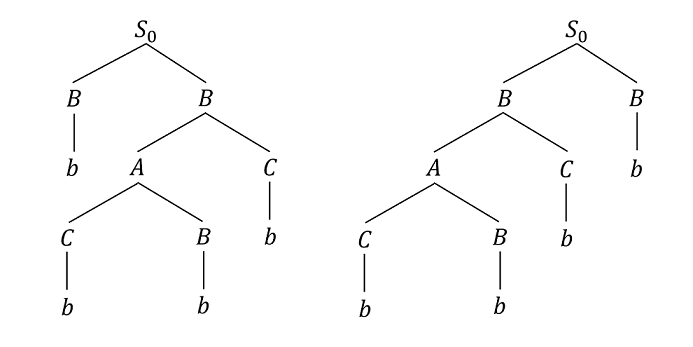
\includegraphics{image2}
\end{center}